\chapter{Application of Theoretical Knowledge}
\label{ch:theory}

\section{Theories, models, frameworks and algorithms relevant to the case}

\subsection{Execution monitoring}
Classical planning separates what a plan intends from what the world shows. PLANEX executed STRIPS plans while comparing each step's expected conditions with the observed state~\cite{fikes1972planex}, and later work on execution monitoring in robotics generalised this to detecting discrepancies at run time~\cite{pettersson2005execution}. The completion gate is a monitor of this kind: the request implies postconditions, and the agent may not declare success until they are observed.

\subsection{Reasoning-and-acting loops as state machines}
A ReAct-style agent~\cite{yao2023react} alternates reasoning, action and observation. Agentic Pilot makes this loop explicit as a finite state machine in LangGraph: eleven nodes, a typed state record, and routing functions that select the next node. Algorithm~1 (Fig.~\ref{fig:alg}) gives the loop. The machine has one accepting transition to \textsc{Completed}, guarded by $\Phi$, so the property ``no task is reported complete unless $\Phi$ held'' follows from the structure of the graph rather than from the model's behaviour.

\begin{figure}[h]
\centering
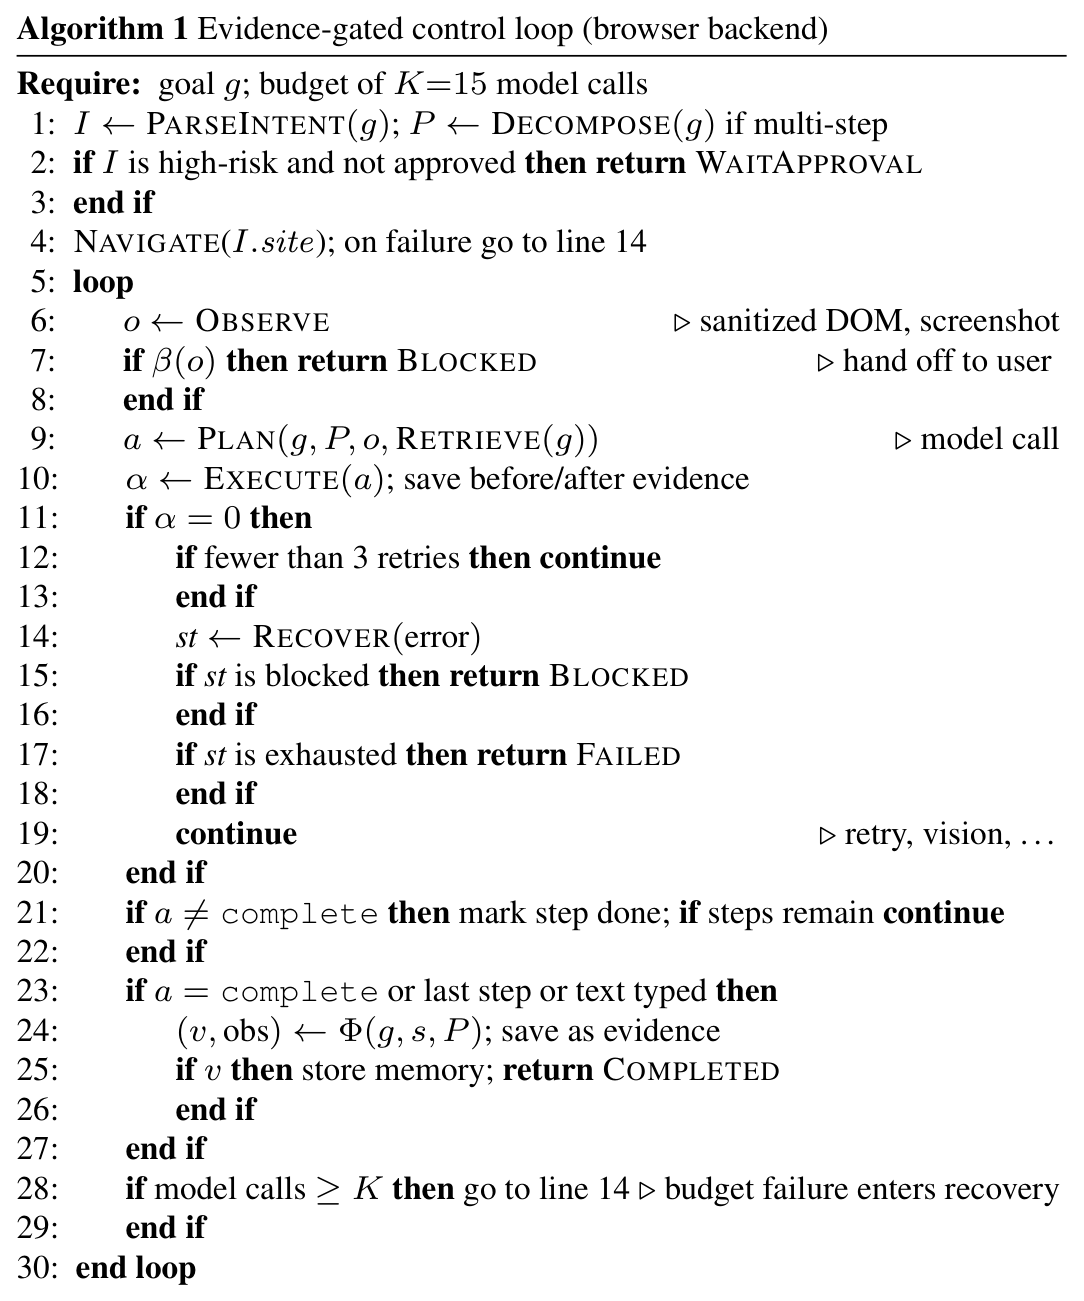
\includegraphics[width=0.85\textwidth]{fig/algorithm.png}
\caption{Algorithm 1: the evidence-gated control loop of Agentic Pilot}
\label{fig:alg}
\end{figure}

\subsection{Conjunctive decision rules and fail-closed design}
$\Phi$ is a conjunction of Boolean checks (Equation~\ref{eq:phi}). A conjunction fails closed: any check that fails, including one that cannot read the page, withholds completion. Adding a conjunct can only reduce false completions and can only raise false rejections, which is why the ablation in Chapter~\ref{ch:analysis} measures both. A rule with no tunable threshold has no ROC curve; its trade-off is characterised by removing conjuncts.

\subsection{Statistical inference for small samples}
The analysis uses methods suited to small counts. The Wilson score interval~\cite{wilson1927probable} behaves better than the normal approximation near 0 and 1; Clopper--Pearson intervals~\cite{clopper1934use} give an exact, conservative check. Paired decisions of two rules on the same states are compared with the exact McNemar test~\cite{mcnemar1947note}, which uses only the discordant pairs: with $b$ states where only the gate is correct and $c$ where only the baseline is correct,
\begin{equation}
p = \min\Bigl(1,\; 2\sum_{i=0}^{\min(b,c)} \binom{b+c}{i}\,2^{-(b+c)}\Bigr).
\end{equation}
For held-out~2 against dispatch-only, $b=9$ and $c=1$ give $p=0.021$. The same formula shows why some tests cannot succeed: with three discordant states the smallest attainable $p$ is 0.25.

\subsection{Monte Carlo simulation with Bayesian rate uncertainty}
The simulation propagates measured rates through the control flow. Each measured rate $k/n$ enters as a Beta posterior, and 1{,}000 scenario sets are regenerated with rates drawn from it, in the spirit of resampling methods~\cite{efron1979bootstrap}. Assumed planner parameters are swept rather than drawn, because no data constrain them.

\subsection{Retrieval-augmented memory}
Memory follows retrieval-augmented generation~\cite{lewis2020rag}: outcomes are stored in a local Chroma collection, embedded with Chroma's default sentence encoder~\cite{reimers2019sbert}, and the nearest records are inserted into later planning prompts. It is evaluated with standard ranking metrics, precision and recall at $k$ and mean reciprocal rank.

\subsection{Security principles}
Three principles apply. \emph{Privacy by design and data minimisation}: inference and records stay on the machine by default. \emph{Least privilege and human approval}: high-risk actions need the user's consent, and CAPTCHAs are left to the user. \emph{Treating page content as untrusted}: element text is sanitised against prompt injection~\cite{greshake2023indirect,liu2024formalizing}.

\section{Mapping of theory to the real-life situation}
Table~\ref{tab:map} maps each theory to where it appears in the case and what it predicted.

\begin{table}[h]
\caption{Mapping of theory to the case}
\label{tab:map}
\small\singlespacing
\begin{tabularx}{\textwidth}{|p{3.1cm}|L|L|}
\hline\hrow \textbf{Theory or model} & \textbf{Where it is used} & \textbf{What it predicts, and what happened}\\\hline
Execution monitoring & Verification node, $\Phi$ & Observed postconditions catch premature claims; held: 9 of 22 held-out claims withheld\\\hline
Finite state machine & LangGraph loop & Only one guarded path to \textsc{Completed}; held in every run\\\hline
Conjunctive, fail-closed rule & Six checks plus $\beta$ & Removing a check raises false completions; held on design states, little effect on held-out states\\\hline
Small-sample inference & Wilson intervals, McNemar & Wide intervals at $n\approx20$; held: 0.23--0.61\\\hline
Monte Carlo with Beta rates & Simulation v2 & Benefit depends on unmeasured inputs; shown by the $\pi$ sweep\\\hline
Retrieval-augmented memory & Chroma memory & Nearest records help planning only if relevant; 3 of 10 top-1 results were not\\\hline
Privacy by design & Loopback enforcement & No non-local connection from the Python processes; held in 70 episodes\\\hline
\end{tabularx}
\end{table}

\section{Course concepts applied}
Table~\ref{tab:course} lists the course concepts that the case applies.

\begin{table}[h]
\caption{Course concepts applied in the case, with justification}
\label{tab:course}
\small\singlespacing
\begin{tabularx}{\textwidth}{|p{3.6cm}|L|}
\hline\hrow \textbf{Concept} & \textbf{How it was applied}\\\hline
Case study method & A real system studied in its setting, with stakeholders, viewpoints and evidence\\\hline
Problem formulation & Gaps G1--G3 and hypotheses H1--H5 stated so that each can be tested\\\hline
Evidence and data analysis & Every number traced to a run record and an evidence class\\\hline
Experimental design & Design and held-out splits; a set frozen before testing; paired comparisons\\\hline
Validation and threats to validity & Recomputation, reproducibility runs, explicit limitations\\\hline
Decision analysis & Alternatives compared and a recommendation justified (Chapter~\ref{ch:insights})\\\hline
Professional ethics & Disclosure of AI assistance; no synthetic result presented as a measurement\\\hline
\end{tabularx}
\end{table}

\section{Where theory and practice differ, and why}

\textbf{Rules generalise less than they appear to.} In theory a postcondition check is exact. In practice, the postconditions are derived from the wording of the request, and new wordings escape them: the gate withheld 20 of 23 unsatisfied design states but 9 of 22 held-out ones. The checks are only as general as the trigger words they recognise.

\textbf{Dispatch is a weak signal even inside the code.} Before the fixes, the live verification node accepted fewer premature claims than the predicate alone, because it let a \texttt{complete} action mark a pending step done and treated the planner's reasoning as an answer. The theory of the predicate was right; the plumbing around it was not.

\textbf{Recovery is less diverse than its taxonomy.} The engine has seven failure types and four strategies, but only vision fallback changes behaviour; the others repeat ordinary planning. A missing confirmation, the failure the gate most often reveals, falls into ``unknown''.

\textbf{Locality is narrower than ``local''.} A loopback endpoint guarantees that prompts are sent to a server on the same machine, not that the server runs inference locally or that the browser itself contacts no other host.
